 \documentclass[12pt,a4paper]{article}

\usepackage{graphicx}% Include figure files
\usepackage{dcolumn}% Align table columns on decimal point
\usepackage{bm}% bold math
%\usepackage{hyperref}% add hypertext capabilities
%\usepackage[mathlines]{lineno}% Enable numbering of text and display math
%\linenumbers\relax % Commence numbering lines

%\usepackage[showframe,%Uncomment any one of the following lines to test 
%%scale=0.7, marginratio={1:1, 2:3}, ignoreall,% default settings
%%text={7in,10in},centering,
%%margin=1.5in,
%%total={6.5in,8.75in}, top=1.2in, left=0.9in, includefoot,
%%height=10in,a5paper,hmargin={3cm,0.8in},
%]{geometry}

\usepackage{multicol}%Para hacer varias columnas
\usepackage{multicol,caption}
\usepackage{multirow}
\usepackage{cancel}
\usepackage{hyperref}
\hypersetup{
    colorlinks=true,
    linkcolor=blue,
    filecolor=magenta,      
    urlcolor=cyan,
}

\setlength{\topmargin}{-1.0in}
\setlength{\oddsidemargin}{-0.3pc}
\setlength{\evensidemargin}{-0.3pc}
\setlength{\textwidth}{6.75in}
\setlength{\textheight}{9.5in}
\setlength{\parskip}{0.5pc}

\usepackage[utf8]{inputenc}
\usepackage{expl3,xparse,xcoffins,titling,kantlipsum}
\usepackage{graphicx}
\usepackage{xcolor} 
\usepackage{siunitx}
\usepackage{nopageno}
\usepackage{lettrine}
\usepackage{caption}
\renewcommand{\figurename}{Figura}
\usepackage{float}
\renewcommand\refname{Bibliograf\'ia}
\usepackage{amssymb}
\usepackage{amsmath}
\usepackage[rightcaption]{sidecap}
\usepackage[spanish]{babel}

\providecommand{\abs}[1]{\lvert#1\rvert}
\providecommand{\norm}[1]{\lVert#1\rVert}
\newcommand{\dbar}{\mathchar'26\mkern-12mu d}

\usepackage{mathtools}
\DeclarePairedDelimiter\bra{\langle}{\rvert}
\DeclarePairedDelimiter\ket{\lvert}{\rangle}
\DeclarePairedDelimiterX\braket[2]{\langle}{\rangle}{#1 \delimsize\vert #2}

% CABECERA Y PIE DE PÁGINA %%%%%
\usepackage{fancyhdr}
\pagestyle{fancy}
\fancyhf{}

\begin{document}

Macías Márquez Misael Iván

\begin{enumerate}



%%%1%%%



\item En la figura 1 se tiene un objeto frente a un espejo plano, dos observadores ven la imagen del objeto en el espacio.¿En cuál de las posiciones de imágenes indicadas ven la imagen cada uno? (A,B,C,D o E)?

\begin{figure}[h!]
    \centering
    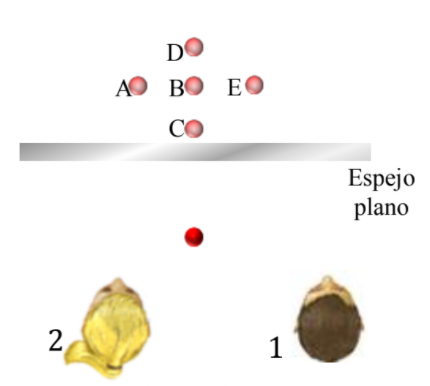
\includegraphics[scale=0.5]{1.PNG}
\end{figure}

\textbf{Res:}

Al tenerse un espejo plano, la imagen virtual del objeto debe estar a la misma distancia del espejo que el objeto real por lo que ambos observadores verán la imagen virtual en el punto D




%%%2%%%



\item Si un objeto está a una distancia de $2f$ de un espejo cóncavo con foco $f$, ¿Cuál es la posición de su imagen?

\textbf{Sol:}

Utilizando la ecuación 5.1 y despejando $o = 2f$:

\begin{equation*}
    \frac{1}{2f} + \frac{1}{i} = \frac{1}{f}
\end{equation*}

\begin{equation*}
    \frac{1}{i } = \frac{1}{f} \left(1 + \frac{1}{2} \right)
\end{equation*}

\begin{equation*}
    \therefore i = 2f
\end{equation*}




%%%3%%%




\item Utilizando la ecuación 5.1, calcular la propagación de la incertidumbre nominal del radio de curvatura $(R)$ y del foco $(f)$ de un espejo, asumiendo que $o$ e $i$ son mediciones experimentales con incertidumbre.

\textbf{Sol:}

Despejando a $R$ de la ecuación 5.1:

\begin{equation*}
    R = \frac{2}{\frac{1}{o} + \frac{1}{i}}
\end{equation*}

y por la regla de derivación para propagación de incertidumbres y la suma por cuadraturas:

\begin{equation*}
    \delta R = \sqrt{\left(\frac{\partial R}{\partial i}\delta i\right)^2 + \left(\frac{\partial R}{\partial o}\delta o\right)^2} = \sqrt{\left(-\frac{2 \delta i}{i^2\left(\frac{1}{o} + \frac{1}{i}\right)^2}\right)^2 + \left(-\frac{2 \delta o}{o^2\left(\frac{1}{o} + \frac{1}{i}\right)^2}\right)^2} 
\end{equation*}

\begin{equation*}
    = \frac{2}{\left(\frac{1}{o} + \frac{1}{i}\right)^2} \sqrt{\frac{\delta i ^2}{i^4} + \frac{\delta o^2}{o^4}} = \frac{R^2}{2} \sqrt{\frac{\delta i^2}{i^4} + \frac{\delta o^2}{o^4}}
\end{equation*}

Ahora despejando a $f$:

\begin{equation*}
    f = \frac{1}{\frac{1}{o} + \frac{1}{i}}
\end{equation*}

y usando el resultado anterior:


\begin{equation*}
     \delta f=  f^2 \sqrt{\frac{\delta i^2}{i^4} + \frac{\delta o^2}{o^4}}
\end{equation*}




%%%4%%%




\item Encontrar la linealización más sencilla de la ecuación 5.1 de forma que a través de una gráfica se pueda encontrar el radio de curvatura o el foco de un espejo cóncavo.

\textbf{Sol:}

Restando $\frac{1}{o}$ en ambos lados de la ecuación 5.1 se tiene:

\begin{equation*}
    \frac{1}{i} = -\frac{1}{o} + \frac{2}{R} = -\frac{1}{o} + \frac{1}{f}
\end{equation*}

que es una linealización donde $y = \frac{1}{i}$, $m=-1$, $x= \frac{1}{o}$ y  $b = \frac{2}{R} = \frac{1}{f}$.


%%%5%%%



\item Utilizando la ecuación 5.4, calcular la propagación de la incertidumbre nominal del radio de curvatura ($R$) de un espejo, asumiendo que $a$ y $h$ son mediciones experimentales con incertidumbres.

\textbf{Sol:}

Por la regla de derivación para propagación de incertidumbres y suma por cuadraturas se tiene que:

\begin{equation*}
    \delta R = \sqrt{\left(\frac{\partial R}{\partial a}\delta a\right)^2 + \left(\frac{\partial R}{\partial h}\delta h\right)^2}
\end{equation*}

\begin{equation*}
    = \sqrt{\left(\frac{2a\delta a}{2h}\right)^2 + \left(-\frac{a^2\delta h}{2h^2} + \frac{\delta h}{2}\right)^2}
\end{equation*}

\begin{equation*}
    = \frac{a}{2h} \sqrt{\delta a^2 + \delta h^2 \left(\frac{a^2}{h^2} + \frac{h^2}{a^2} -2\right)}
\end{equation*}

    
    
\end{enumerate}

\end{document}